
\section*{États des Processus et Diagramme d'État}

Les processus dans un système d'exploitation passent par plusieurs états :

\begin{itemize}
    \item \textbf{EX (Exécution)}
    \item \textbf{PR (Prêt)}
    \item \textbf{BL (Bloqué)}
    \item \textbf{EM (En Mémoire)}
    \item \textbf{HM (Hors Mémoire)}
\end{itemize}


\begin{figure}[h]
    \centering
    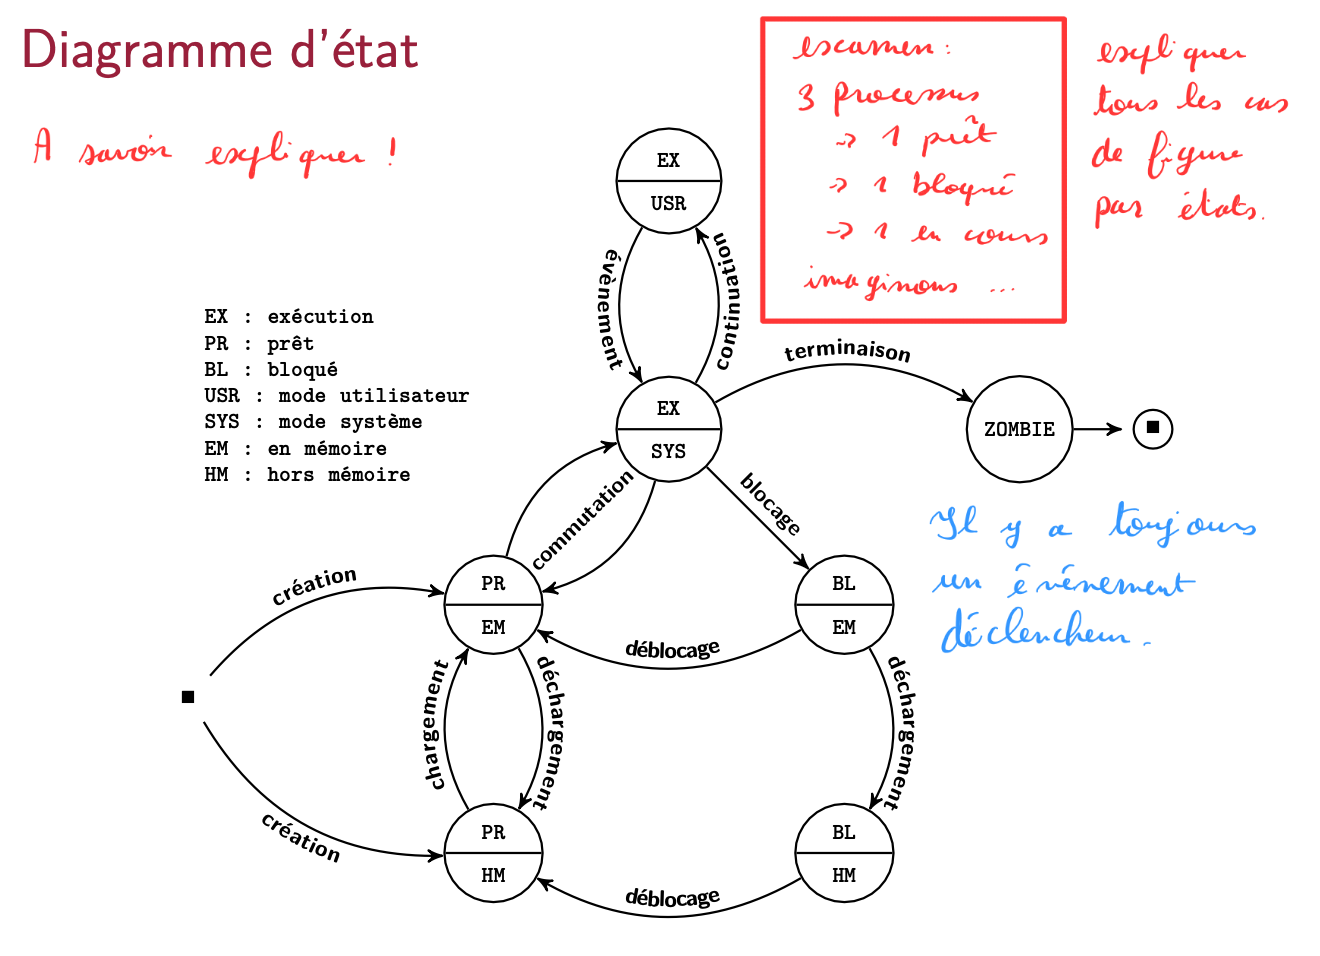
\includegraphics[width=0.8\textwidth]{Images/Diagrams/schema.png}
    \caption{Process}
\end{figure}

Chaque transition d'un état à un autre peut être déclenchée par divers événements, tels que des interruptions, des appels système, des fautes de pages, etc.

\section*{Cas de Figure avec Trois Processus}

Imaginons trois processus avec les états suivants :

\begin{itemize}
    \item \textbf{P1 (en cours)} : EX (Exécution)
    \item \textbf{P2 (prêt)} : PR (Prêt)
    \item \textbf{P3 (bloqué)} : BL (Bloqué)
\end{itemize}

Nous allons examiner les transitions possibles entre ces états en prenant en compte la protection/projection de la mémoire et la pagination.

\subsection*{1. Transition de P1 (EX) à P2 (PR)}

\textbf{Cause :} Fin du quantum de temps (dans un algorithme de round-robin), ou une interruption I/O.

\begin{itemize}
    \item \textbf{Algorithme d'Ordonnancement :} Utilisation de l'algorithme Round-Robin.
    \item \textbf{Projection/Protection :} Les tables de pages de P2 sont projetées en mémoire principale (MP) si nécessaire, avec des mécanismes de protection pour assurer que seules les pages de P2 sont accessibles.
    \item \textbf{Pagination :} Si une page nécessaire n'est pas en mémoire, un défaut de page est déclenché, et la page est chargée à partir de la mémoire secondaire.
\end{itemize}

\textbf{Transition :} P1 passe de EX à PR, P2 de PR à EX.

\textbf{État final :} P1 (PR), P2 (EX), P3 (BL).

\subsection*{2. Transition de P2 (EX) à P3 (BL)}

\textbf{Cause :} P2 demande une opération I/O et doit attendre la fin de cette opération.

\begin{itemize}
    \item \textbf{Algorithme d'Ordonnancement :} Le processus suivant prêt à être exécuté est sélectionné (par exemple, P1).
    \item \textbf{Projection/Protection :} Les pages de P3 peuvent être projetées en mémoire principale si nécessaires, et les pages de P2 peuvent être déplacées vers le disque.
    \item \textbf{Pagination :} Les pages non utilisées de P2 peuvent être paginées vers le disque.
\end{itemize}

\textbf{Transition :} P2 passe de EX à BL, P1 de PR à EX.

\textbf{État final :} P1 (EX), P2 (BL), P3 (BL).

\subsection*{3. Transition de P3 (BL) à P1 (PR)}

\textbf{Cause :} L'événement attendu par P3 (fin d'une opération I/O) se produit.

\begin{itemize}
    \item \textbf{Algorithme d'Ordonnancement :} Le processus suivant prêt à être exécuté est sélectionné.
    \item \textbf{Projection/Protection :} Les pages de P3 peuvent être projetées en mémoire principale si nécessaires.
    \item \textbf{Pagination :} Si les pages de P3 avaient été paginées, elles sont rechargées en mémoire.
\end{itemize}

\textbf{Transition :} P3 passe de BL à PR, P1 de EX à PR.

\textbf{État final :} P1 (PR), P2 (BL), P3 (PR).

\section*{Protection/Projection de la Mémoire}

La protection et la projection de la mémoire sont des concepts clés pour garantir que chaque processus accède uniquement à sa propre mémoire. Cela est réalisé grâce aux tables de pages et aux mécanismes de protection matérielle comme les registres de contrôle et les modes de privilège du processeur.

\begin{itemize}
    \item \textbf{Tables de Pages :} Utilisées pour mapper les adresses virtuelles aux adresses physiques.
    \item \textbf{Mécanismes de Protection :} Utilisation de bits de contrôle pour empêcher les accès non autorisés.
    \item \textbf{Basculement de Stack :} Lorsqu'une interruption ou un événement se produit, le système peut basculer sur une stack dédiée pour le gestionnaire d'événements.
\end{itemize}

\section*{Pagination}

La pagination est utilisée pour gérer la mémoire de manière efficace, en divisant la mémoire en blocs de taille fixe appelés pages. Lorsque la mémoire physique est pleine, certaines pages peuvent être déplacées vers le disque dur (mémoire secondaire).

\begin{itemize}
    \item \textbf{Défaut de Page :} Se produit lorsqu'une page demandée n'est pas en mémoire. Le système doit alors charger cette page à partir du disque, ce qui peut entraîner une transition d'état.
    \item \textbf{Algorithmes de Remplacement de Pages :} LRU (Least Recently Used), FIFO (First In First Out), NRU (Not Recently Used), et Seconde Chance. Ces algorithmes déterminent quelles pages doivent être remplacées lorsqu'une nouvelle page doit être chargée.
\end{itemize}

\section*{Diagramme d'État avec Cas de Figure}

Un diagramme d'état peut être utilisé pour illustrer ces transitions. Chaque état et transition doit être clairement indiqué avec les événements correspondants qui déclenchent les transitions.

\textbf{Exemple de Transitions :}

\begin{itemize}
    \item \textbf{EX à PR :} Fin de quantum, interruption.
    \item \textbf{PR à EX :} Sélection par l'ordonnanceur.
    \item \textbf{EX à BL :} Demande I/O.
    \item \textbf{BL à PR :} Fin d'une opération I/O.
\end{itemize}

\section*{Conclusion}

Cette explication couvre les transitions d'état des processus en tenant compte des algorithmes d'ordonnancement, de la protection/projection de la mémoire, et de la pagination. Chaque transition est déclenchée par des événements spécifiques, et la gestion de la mémoire est cruciale pour assurer une exécution efficace et sécurisée des processus. Les algorithmes de remplacement de pages jouent un rôle clé dans la gestion de la pagination pour optimiser l'utilisation de la mémoire physique disponible.
